\newpage
\section{Arkitektur}

\begin{figure}[H]
    \makebox[\textwidth][c]{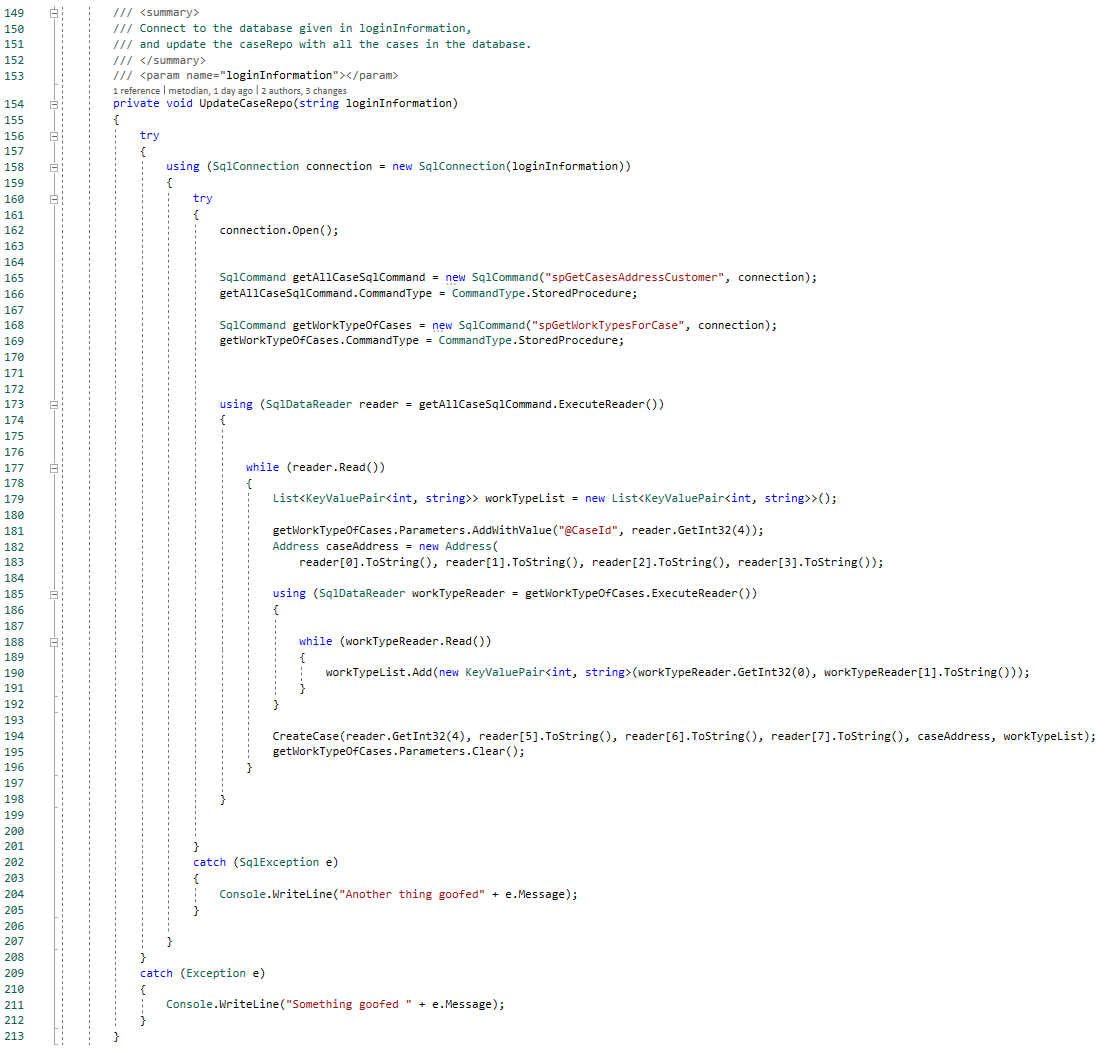
\includegraphics[scale = 0.8]{UpdateCaseRepo.PNG}}
    \caption{Her vises metoden UpdateCaseRepo, som ligger i classen CaseRepo. Denne metoder henter alle cases med til hørende customers og addresses fra databasen.}
    \label{fig:UpdateCaseRepo}
\end{figure}

I figur \ref{fig:UpdateCaseRepo} ser vi opdaterings metode som sørger for at hente alle vores cases fra databasen. UpdateCaseRepo tager som parameret en string og denne string indeholder login informationer til den database vi bruger, dette kan ses på linje 154.
Det første vi gør er at vi bruger en try og catch på Sqlconnection, for at se om vi kan lave en connection med den string metoden bruger. Hvis den ikke kan lave en Sqlconnection fanger catchen den exeception der blive smidt ud. I linje 158 bruges der keyworded using, som sørger at lukke Sqlconnection igen efter den er færdig med at bruge den, ellers skal metoden Close() bruges for at lukke forbindelen.
\\
Efter forbindelsen er blevet åbnet med metoden Open() i linje 162, bliver der lavet to Sqlcommands (getAllCasesSqlcommand og getWorkTypeOfCases) fra linje 165 til 169. Som bliver defineret som stored procedures.[ref storedprocedures]
\\
I linje 173 bliver der brugt en ny using hvor der bliver oprettet og eksekveret en SqlDataReader på Sqlcommanden getAllCasesSqlcommand. Efterfølgende bruges der et while loop som kører hele readeren igennem, med metoden Read() dette sker i linje 177. Inde i dette while loop bliver der oprettet en ny liste workTypeList, som er af typen KeyValuePair.
Før den næste Sqlcommand getWorkTypeOfCases bliver kørt bliver der først lavet en parameret, som denne Sqlcommand bruger og denne parameret kommer fra den første Sqlcommand getAllCasesSqlcommand. Hvor der samtidlig bliver lavet et addresse objekt udfra de outputs der kommer fra getAllCasesSqlcommand.
\\
getWorkTypeOfCases bliver eksikveret hvor den går ind og tilføger og opretter ny keyValuePair til listen workTypeList.
\\
Til sidste før at loopet bliver kørt igen bliver der oprettet et nyt case objeckt, men de resterende outputs fra  getWorkTypeOfCases og de nye objekter der er blevet lavet.
For at kunne blive ved at bruge de samme parametre er man nød til at bruge metoden Clear() til sidste for ellers kan man ikke oprette en ny parameter med samme navn den den allerede eksistere.
